\documentclass[letterpaper,spanish,11pt]{article}
\usepackage[utf8]{inputenc}    % Agregar y acentos
\usepackage{babel}               % Soporte multilenguajes
%\usepackage{avant}               % Tipo de fuente
%\usepackage{fancyheadings}       %% Topes y pies de p�ina
%\usepackage[dvips]{graphicx}     % Inclusion de imagenes .eps
\usepackage{amsmath,amsthm,url}
%\usepackage{url}                 % Agregar Links soporte de ~
\usepackage{verbatim}
%\usepackage{geometry}
\usepackage{color}
\usepackage{amsfonts}
\usepackage{amssymb}
%\usepackage{txfonts}
%\usepackage{pxfonts}
%\usepackage{fancybox}
\usepackage{latexsym}
%\usepackage{fancyvrb}
\usepackage{graphicx}
%\usepackage{pstricks}
\usepackage{setspace} % paquete para interlineado
\usepackage{url}
\usepackage{colortbl}
\usepackage{multirow}
\usepackage{slashbox}
\usepackage{rotating}
\definecolor{rojo}{rgb}{1,0,0}
\oddsidemargin -0.1in
\topmargin -0.5in
\textwidth 6.7in
\textheight 8.5in

\begin{document}

\begin{titlepage}
%\begin{figure}[htbp]
\begin{center}

\includegraphics[height=3.5cm]{images/logo_latex}
\end{center}
%\end{figure}
\vspace{1.5cm}
\begin{center}
\textbf{\Huge{Laboratorio de estad\'istica}}\\[0.2cm]
\textbf{\Huge{computacional}}\\[0.7cm]
\textbf{\huge{Informe \# 4}}\\[0.7cm]
\textbf{\huge{``Intervalos de confianza''}}\\[0.3cm] 
\today\\[1.5cm]
\end{center}
\vspace{2cm}
\begin{flushright}
\large{\textbf{Profesor de C\'atedra}} \\
\large{Ricardo \~{N}anculef} \\[0.5cm]
\large{\textbf{Ayudantes de laboratorio}}\\
\large{Milciades Reyes}\\
\large{Fernando Herrera}\\[0.5cm]
\large{\textbf{Integrantes}} \\
\large{Esteban Bombal 2673004-k} \\
\large{Rodrigo Fernandez 2673002-3} \\
\large{Cristian Maureira 2673030-9} \\
\large{Gabriel Zamora 2673070-8} \\
\end{flushright}
\end{titlepage}

\section{Descripci\'on del Fen\'omeno y del Muestreo}

\begin{enumerate}
\item A partir de su observaci\'on de la poblaci\'on, formule hip\'otesis acerca del fen\'omeno que estudia.

\begin{itemize}
	\item Hipotesis: ''Los cigarros light duran menos en ser fumados que los cigarros corrientes (filtro cafe)''
\end{itemize}

\item Una estaci\'on de radio muy popular recibe muchas llamadas en el d\'ia de tal forma que la probabilidad
de que una persona llame a la radio y la l\'inea de tel\'efono no este ocupada es 0.05. suponga que las
llamadas son independientes.
% Geometrica
% P = 0.05 , en promedio, 1 contesta cada 20 llamadas

\begin{itemize}
	\item Lea las siguientes preguntas y escriba sus hip\'otesis.
	\item ?`Cu\'al es la probabilidad de que la primera llamada que entre sea la d\'ecima que realiza la persona?\\
		Como en la Geometrica se realizan X + 1 experimentos para obtener ese 1 exito, para que entre la decima, nuestro $X=9$\\
		$p(X=9)\ =\ 0.03151247$\\% dgeom(9,0.05)
	\item ?`Cu\'al es la probabilidad de que sea necesario llamar mas de 15 veces para que encuentro la l\'inea desocupada?\\
		En este caso $X>15$, entonces necesitamos saber $X<=15$\\
		$P(X>15)\ =\ 1\ -\ P(X<=15)\ =\ 1\ -\ 0.5598733\ =\ 0.4401267\ $\\ %pgeom(15,0.05)
	\item ?`Cu\'al es el n\'umero esperado de llamadas que tiene que realizar una persona para hallar desocupada la l\'inea?.
		 Calcule utilizando el o los par\'ametros de la distribuci\'on y usando $\sum_{i=1}^{100}x\cdot p(x)$, comp\'arelos y explique por qu\'e la diferencia.\\
	$$\bar{x}\ =\ E(x)\ =\ \frac{1}{\lambda} =\ \frac{1}{0.05} =\ 20$$
	y si ahora comparamos  eso con:\\
	$$\sum_{i=1}^{100}x\cdot p(x)\ =\ 19.20401$$
	
	Nos podemos dar cuenta que la diferencia es de $0.8$ , el cual representa el error al calcular la esperanza tomando en cuenta solo 100 llamadas. La diferencia reside en que la formula de la esperanza considera la suma integral de todos los valores de 0 a infinito. De hecho, si en vez de calcularla con x=1 a 100, lo hacemos hasta 10000, la diferencia se reduce a $0.005$, una diferencia \'infima comparada con el valor entregado por la formula.

	\item Realice gr\'aficos de la funci\'on de densidad de probabilidad y de la funci\'on de distribuci\'on.\\
		% x<-seq(1,40)
	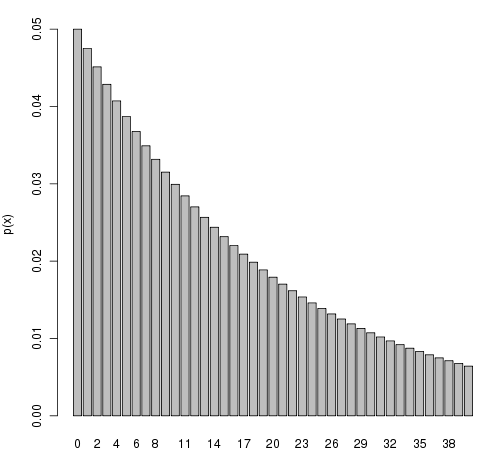
\includegraphics[scale=0.5]{images/1_2-dgeom}\\	% barplot(dgeom(x,0.05),names.arg=x)
	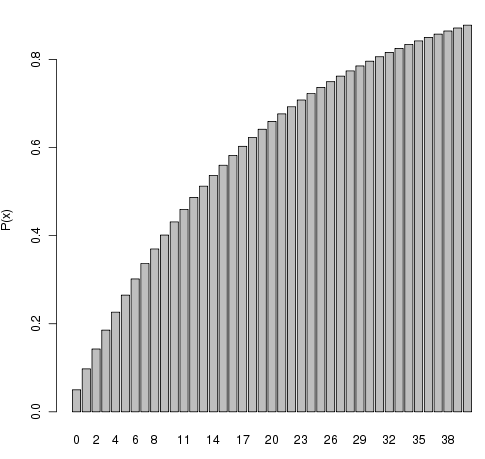
\includegraphics[scale=0.5]{images/1_2-pgeom}\\	% barplot(pgeom(x,0.05),names.arg=x)
	\item Var\'ie el o los valores de los par\'ametros de la distribuci\'on y comente lo observado en los gr\'aficos de la funci\'on de densidad y de distribuci\'on. (2 casos)\\\\

	Caso 1: Variando el $\lambda$ a $0.1$:\\
	Funci\'on de densidad de probabilidad con $\lambda\ =\ 0.1$\\
  	  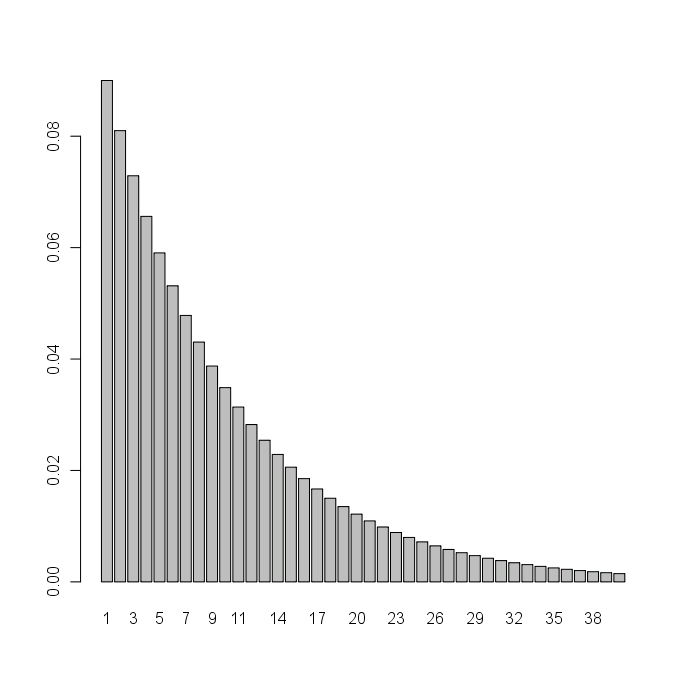
\includegraphics[width=3.3in,height=3.3in]{images/1_2-dgeom01.png}\\
	Funci\'on de distribucion con $\lambda\ =\ 0.1$\\
  	  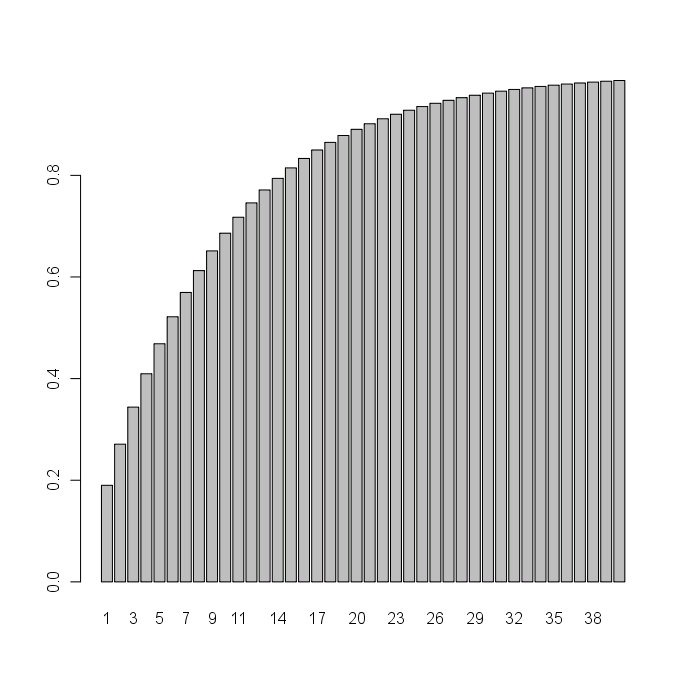
\includegraphics[width=3.3in,height=3.3in]{images/1_2-pgeom01.png}\\
	Caso 2: Variando el $\lambda$ a $0.5$:\\
	Funci\'on de densidad de probabilidad con $\lambda\ =\ 0.1$\\
  	  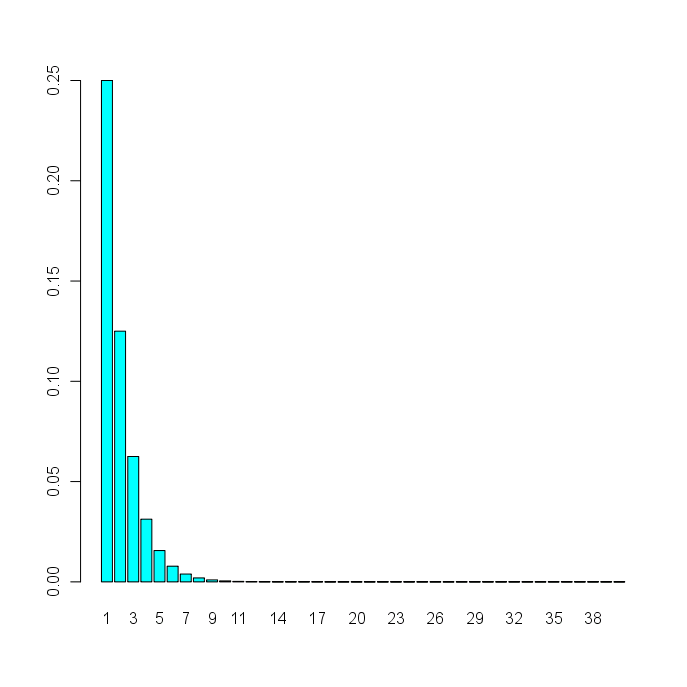
\includegraphics[width=3.3in,height=3.3in]{images/1_2-dgeom5.png}\\
	Funci\'on de distribucion con $\lambda\ =\ 0.1$\\
  	  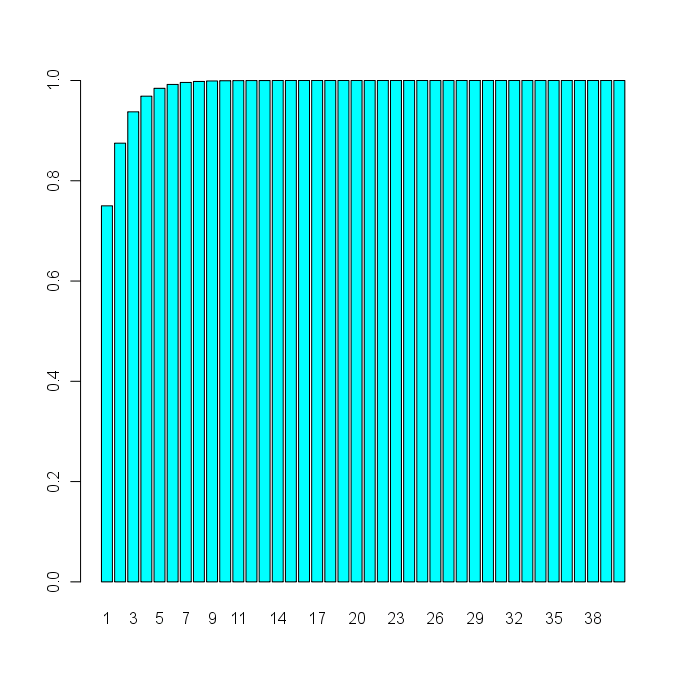
\includegraphics[width=3.3in,height=3.3in]{images/1_2-pgeom5.png}\\

	Claramente podemos observar como al aumentar el parametro $\lambda$, la funcion de densidad y distribucion tiende a comprimirse y aumentar de valor.
  De la misma forma, uno puede notar como la pendiente de las funciones se pronuncia (negativamente en la de densidad y positivamente en la de distribuci\'on) considerablemente al aumentar $\lambda$.

	


\end{itemize}

\item Definir y justificar una metodolog\'ia de muestreo.
	\begin{itemize}
		\item Decidimos proceder la toma de muestreo precisamente en los lugares de descansos mas concurridos de la UTFSM, ll\'amese Patio Central, Patio del Ca~n\'on, entradas del Edificio C, etc. \\
		Nuestro punto es que registrar nuestra muestra dentro de nuestra Universidad presenta varios beneficios, por ejemplo, que la misma toma de muestras resulta menos invasiva para la poblaci\'on, al encontrarnos dentro de un recinto donde la toma de muestras y los datos son comunes. \\
		Otro tema es el uso de los datos. Aparte de comprobar \'esta hipotesis, podemos estudiar varias otras hipotesis de inter\'es comunitario, como el grado de stress que presentan los alumnos frente a los cert\'amenes finales, segun el tiempo en que se demoran en fumarse un cigarro, lo cual no haremos en este momento por tratarse de un informe sobre otros m\'etodos.
	\end{itemize}

\item En un local de lavado de autos ``CarLimpio'' se lava un auto a al vez, lo cual produce una cola de autos esperando ser atendidos.
La tasa de tiempo entre llegadas de autos a la cola es de 10 minutos, donde la llegada de un auto es independiente de la llegada de otro.
% Poisson
% llega 1/10 auto/min, = 0.1 auto/min = 6 auto/hora
\begin{itemize}
	\item ?`Cu\'al es la esperanza y varianza de llegada de autos a la cola por hora?\\
		$Esperanza\ =\ E(x)\ =\ \lambda\ =\ 6$\\
		$Varianza\ =\ V(x)\ =\ \lambda\ =\ 6$\\
	\item ?`Cu\'al es la probabilidad de que lleguen 5 autos en una hora?\\
		$P(X=5)\ =\ 0.1606231\ $\\ % dpois(5,6)
	\item ?`Cu\'al es la probabilidad de que lleguen mas de 7 autos en una hora?\\
		$P(X>7)\ =\ 1\ -\ P(X<=7)\ =\ 1\ -\ 0.7439798\ =\ 0.2560202\ $\\ %1 - ppois(7,6)
	\item Realice gr\'aficos de la funci\'on de densidad de probabilidad y de la funci\'on de distribuci\'on.\\
		%x<-seq(1,40) ; supongo que se le pueden dar cualquier valor, total hay que ver como se comporta...de 1 a 40 pienso que esta bien
		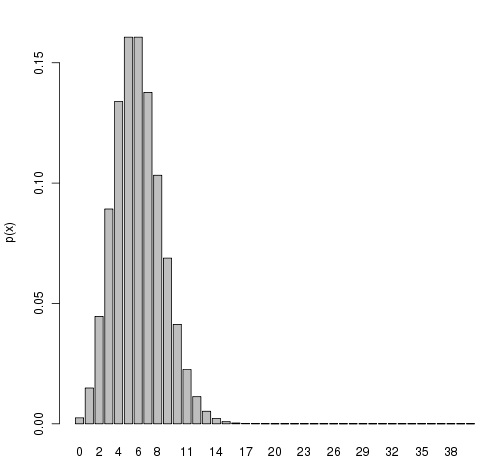
\includegraphics[scale=0.5]{images/1_4-dpois} \\%barplot(dpois(x,6),names.arg=x) 
		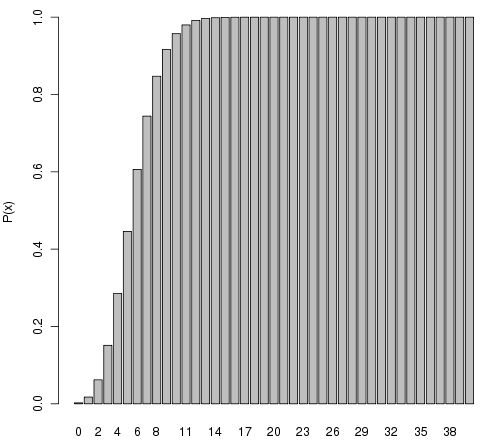
\includegraphics[scale=0.5]{images/1_4-ppois} \\%barplot(ppois(x,6),names.arg=x)
	\item Var\'ie el o los valores de los par\'ametros de la distribuci\'on y comente lo observado en los gr\'aficos de la funci\'on de densidad y de distribucii\'on. (2 casos)\\

	Caso 1: Variando el $\lambda$ a $20$:\\
	Funci\'on de densidad de probabilidad con $\lambda\ =\ 20$\\
  	  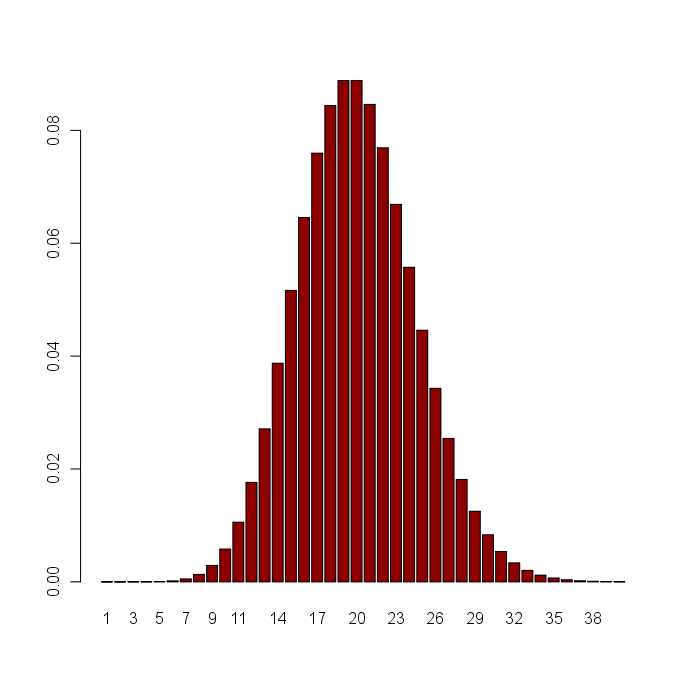
\includegraphics[width=3.3in,height=3.3in]{images/1_4-dpois20.png}\\
	Funci\'on de distribucion con $\lambda\ =\ 20$\\
  	  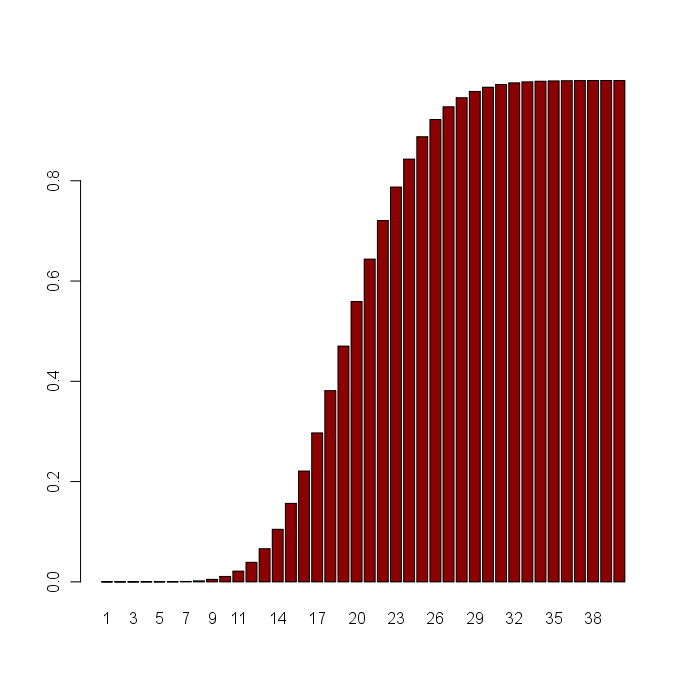
\includegraphics[width=3.3in,height=3.3in]{images/1_4-ppois20.png}\\
	Caso 2: Variando el $\lambda$ a $40$:\\
	Funci\'on de densidad de probabilidad con $\lambda\ =\ 40$\\
  	  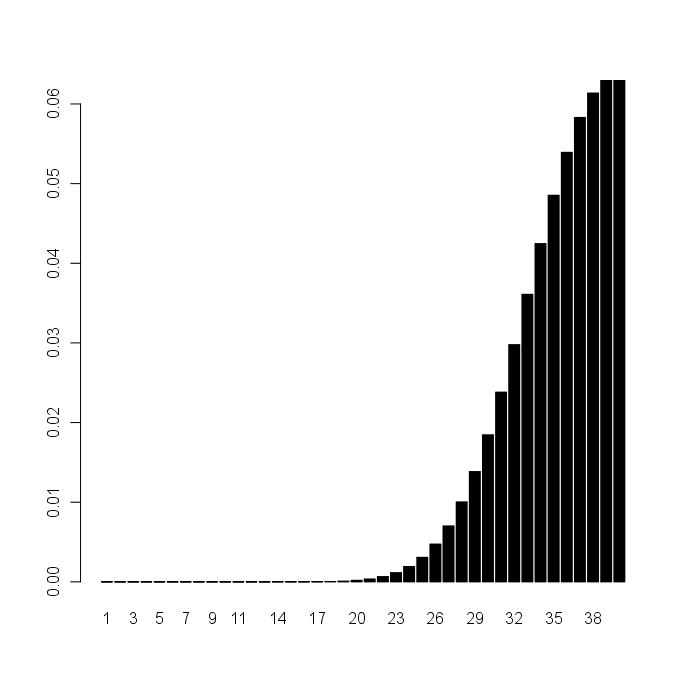
\includegraphics[width=3.3in,height=3.3in]{images/1_4-dpois40.png}\\
	Funci\'on de distribucion con $\lambda\ =\ 40$\\
  	  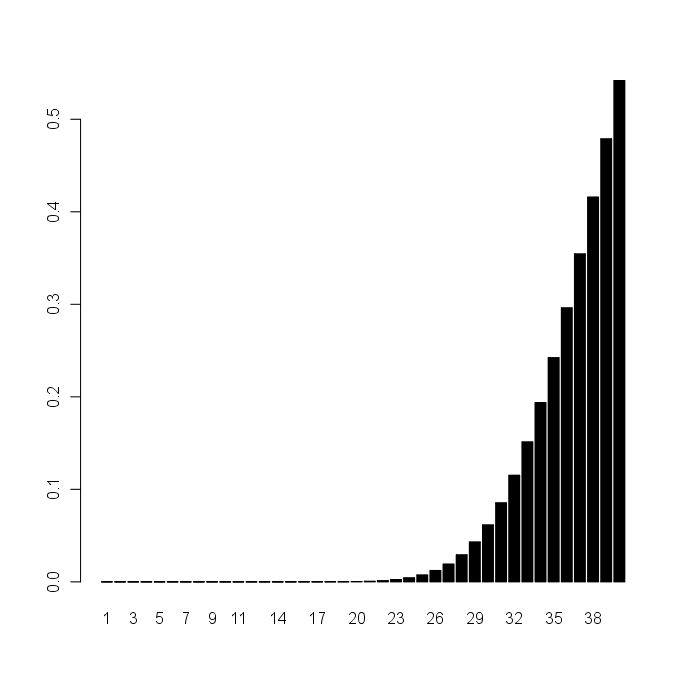
\includegraphics[width=3.3in,height=3.3in]{images/1_4-ppois40.png}\\

	Claramente podemos observar como al aumentar el parametro $\lambda$, la funcion de densidad y distribucion tiende a desplazarse hacia la derecha y ir disminuyendo la probabilidad maxima alcanzada.

\end{itemize}

\end{enumerate}

\section{Intervalos de confianza}

\begin{enumerate}
\item Calcular el intervalo de confianza de tiempo promedio de los cigarros tipo light, con un 75 \%, 85 \% y
95 \% de confianza. (hint: varianza poblacional desconocida).

Teniendo en cuenta que:\\

$P(\overline{x} - t_{1-\frac{\alpha}{2}}\frac{\widehat{\sigma}}{\sqrt{n}} \leq \mu_x \leq \overline{x} + t_{\frac{\alpha}{2}}\frac{\widehat{\sigma}}{\sqrt{n}}) = 1 - \alpha$\\
$\overline{x} = 381.244$\\
$\widehat{\sigma} = 58.55714$\\
$n = 50$\\
t = Distribucion t-student con n-1 grados de libertad\\

Por lo que: \\

\begin{itemize}

\item $\alpha = 0.25$

$\mu_x \in$ [371.50399 , 390.98581]

\item $\alpha = 0.15$

$\mu_x \in$ [369.00691 , 393.48288]

\item $\alpha = 0.05$

$\mu_x \in$ [364.42532 , 398.06447]

\end{itemize}

\item Calcule los intervalos de confianza anteriores suponiendo que el tama\~no de la muestra es el doble y el
triple. (manteniendo el mismo tiempo promedio y varianza muestral).

Teniendo en cuenta que: \\

n = 100\\

Por lo que: \\

\begin{itemize}

\item $\alpha = 0.25$

$\mu_x \in$ [374.3994 , 388.0904]

\item $\alpha = 0.15$

$\mu_x \in$ [372.66186 , 389.82793]

\item $\alpha = 0.05$

$\mu_x \in$ [369.50493 , 392.98486]

\end{itemize}

Teniendo en cuenta que: \\

n = 150\\

Por lo que: \\

\begin{itemize}

\item $\alpha = 0.25$

$\mu_x \in$ [375.66685 , 386.82295]

\item $\alpha = 0.15$

$\mu_x \in$ [374.25560 , 388.23419]

\item $\alpha = 0.05$

$\mu_x \in$ [371.69972 , 390.79008]

\end{itemize}

\item Calcule los intervalos de confianza del punto 1, suponiendo que la varianza poblacional es igual a la
varianza muestral ($\sigma$ = S), es decir. con varianza poblacional conocida. ?`es mucha la diferencia?

Teniendo en cuenta que: \\

$\overline{x} = 381.244$\\
$\widehat{\sigma} = 58.55714$\\
$n = 50$\\

Por lo que: \\

\begin{itemize}

\item $\alpha = 0.25$

$\mu_x \in$ [371.62187 , 390.86792]

\item $\alpha = 0.15$

$\mu_x \in$ [369.20278 , 393.28702]

\item $\alpha = 0.05$

$\mu_x \in$ [364.84920 , 397.64060]

\end{itemize}


La diferencia es a nivel decimal, por lo tanto no afecta tanto, en situaciones aproximadas.

\item Calcular el intervalo de confianza de tiempo promedio de los cigarros con filtro color caf\'e, con un 75 \%,
85 \% y 95 \% de confianza.

Teniendo en cuenta que: \\

$P(\overline{y} - t_{1-\frac{\alpha}{2}}\frac{\widehat{\sigma}}{\sqrt{n}} <= \mu_y <= \overline{y} + t_{\frac{\alpha}{2}}\frac{\widehat{\sigma}}{\sqrt{n}}) = 1 - \alpha$\\
$\overline{y} = 399.6327$\\
$\widehat{\sigma} = 48.83462$\\
$n = 50$\\
t = Distribucion t-student con n-1 grados de libertad\\

Por lo que: \\

\begin{itemize}

\item $\alpha = 0.25$

$\mu_y \in$ [391.50907 , 407.75624]

\item $\alpha = 0.15$

$\mu_y \in$ [389.42660 , 409.83871]

\item $\alpha = 0.05$

$\mu_y \in$ [385.60571 , 413.65960]

\end{itemize}

\item %
% PARECE QUE ESTA LISTA, REVISAR
%

La edad a la que un hombre contrae matrimonio por primera vez es una variable aleatoria con distribuci\'on gamma.
Si la edad promedio es de 30 a\~nos y los mas com\'un es que el hombre se case a los 22 a\~nos.
% Gamma
% Media = 30 anios
% Moda = 22 anios 
\begin{itemize}
	\item Encontrar los par\'ametros de forma y escala de la distribuci\'on.\\

	Aca nos interesa encontrar cuanto es el tiempo esperado en que un hombre se case.
	Nos dicen que la edad promedio (el cual podemos considerar como nuestro $\lambda$) es de 30 a\~nos,
	y como nos interesa saber cuando un hombre se casa ''por primera vez``, tomamos a $\alpha = 1$. Ahora:
	Sabemos que la media de una distribuci\'on $\Gamma$ es igual a:
	$$\bar{x}\ =\ E(x)\ =\ \frac{\lambda}{\alpha}\ =\ 30$$
	y sabemos que la moda de una distribuci\'on $\Gamma$ es igual a:
	$$Moda\ =\ \frac{\lambda-1}{\alpha}\ =\ 22\ \ \ \ \ si\ \lambda>1$$
	Por lo que resolviendo el sistema de ecuaciones, nos queda $\lambda = 26.5$\\
	
	$$\therefore\ p(t)\ =\ \frac{\lambda^{\alpha}t^{\alpha-1}e^{-\lambda t}}{\Gamma(\alpha)}\ =\ \frac{26.5\cdot e^{-t}}{\Gamma(1)} $$
	
	\item ?`Cu\'al es la probabilidad de que un hombre se case despu\'es de los 25 a\~nos?\\
	$$\therefore\ p(t>25)\ =\ 1-p(t<25)\ =\ 1\ -0.6106966\ =\ 0.3893034$$

	\item Grafique la funci\'on de densidad de probabilidad y de distribuci\'on.\\\\
	Funci\'on de densidad de probabilidad:\\
  	  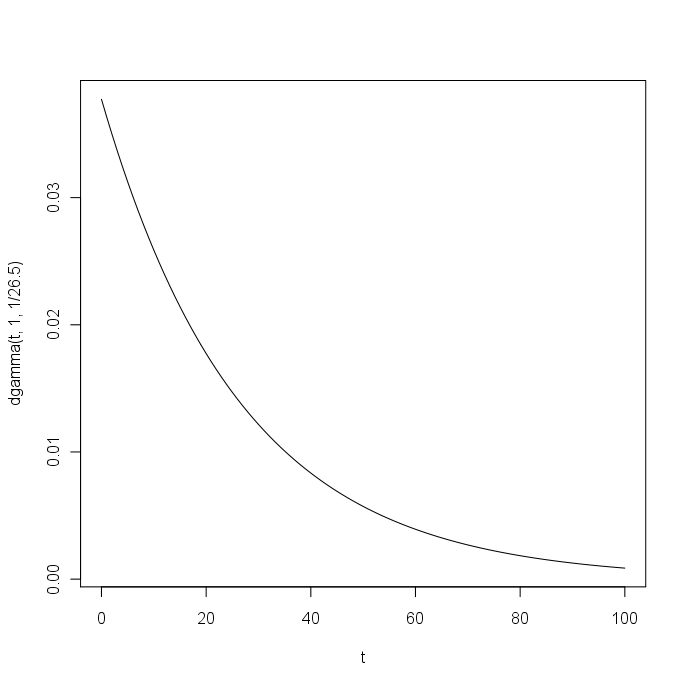
\includegraphics[width=3.3in,height=3.3in]{images/2_5-dgamma.png}\\
	Funci\'on de distribucion:\\
  	  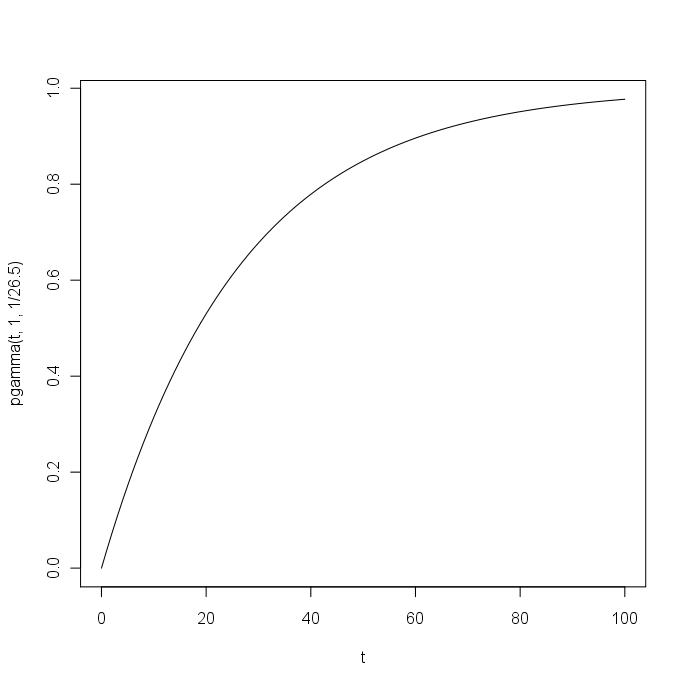
\includegraphics[width=3.3in,height=3.3in]{images/2_5-pgamma.png}
	
\end{itemize}

\item Calcular el intervalo de confianza para la varianza del tiempo de duraci\'on del cigarro de tipo light, con
un 75 \%, 85 \% y 95 \% de confianza.

Teniendo en cuenta que: \\

$P(\frac{\sum(x_i - \overline{x})^2}{\chi_{1-{\frac{\alpha}{2}}}^2} <= \sigma^2 <= \frac{\sum(x_i - \overline{x})^2}{\chi_{\frac{\alpha}{2}}^2}) = 1 - \alpha$\\

$\widehat{s}^2 = \sum \frac{(x_i - \overline{x})^2}{n-1}$\\

$\Leftrightarrow P(\frac{\widehat{s}^2 (n-1)}{\chi_{1-{\frac{\alpha}{2}}}^2} <= \sigma^2 <= \frac{\widehat{s}^2 (n-1)}{\chi_{\frac{\alpha}{2}}^2}) = 1 - \alpha$

$\widehat{s}^2 = 3428.939$\\
$n - 1 = 49$\\
$\chi^2$ = distribucion chi-cuadrado con n-1 grados de libertad\\

Por lo que: \\

\begin{itemize}

\item $\alpha = 0.25$

$\sigma^2 \in$ [2770.269 , 4446.106]

\item $\alpha = 0.15$

$\sigma^2 \in$ [2623.445 , 4744.634]

\item $\alpha = 0.05$

$\sigma^2 \in$ [2384.568 , 5351.706]

\end{itemize}

\item Calcular el intervalo de confianza para la varianza del tiempo de duraci\'on del cigarro con filtro color
caf\'e, con un 75 \%, 85 \% y 95 \% de confianza.

Teniendo en cuenta que: \\

$P(\frac{\sum(y_i - \overline{y})^2}{\chi_{1-{\frac{\alpha}{2}}}^2} <= \sigma^2 <= \frac{\sum(y_i - \overline{y})^2}{\chi_{\frac{\alpha}{2}}^2}) = 1 - \alpha$\\

$\widehat{s}^2 = \sum \frac{(y_i - \overline{y})^2}{n-1}$\\

$\Leftrightarrow P(\frac{\widehat{s}^2 (n-1)}{\chi_{1-{\frac{\alpha}{2}}}^2} <= \sigma^2 <= \frac{\widehat{s}^2 (n-1)}{\chi_{\frac{\alpha}{2}}^2}) = 1 - \alpha$

$\widehat{s}^2 = 2384.821$\\
$n - 1 = 49$\\
$\chi^2$ = distribucion chi-cuadrado con n-1 grados de libertad\\

Por lo que: \\

\begin{itemize}

\item $\alpha = 0.25$

$\sigma^2 \in$ [1926.717 , 3092.259]

\item $\alpha = 0.15$

$\sigma^2 \in$ [1824.601 , 3299.884]

\item $\alpha = 0.05$

$\sigma^2 \in$ [1658.463 , 3722.101]

\end{itemize}

\item ?`Se puede decir que el cigarro light presentan mayor duraci\'on?. fundamente, use $\alpha$ = 0,05.
	\begin{itemize}
		\item Como podemos apreciar, comparando los intervalos de confianza de tiempo promedio de los cigarros light y corrientes. Los cigarros corrientes presentan un limite superior e inferior mayores que los cigarros light, con una diferencia de unos 20 segundos app. Esto quiz\'as se deba a que al ser mas fuerte el cigarro corriente, la gente se demora mas en terminarlo por lo general.\\\\
	Intervalos de Confianza de tiempo Promedio\\
        \begin{tabular}{|c|c|c|}\hline

         & Cigarro Light & Cigarro Corriente\\\hline
        $\mu$ & [$364$ , $398$] & [$391$ , $407$] \\\hline
        \end{tabular}

	
	\end{itemize}

\item Escriba conclusiones a partir de los resultados anteriores, tomen en cuenta el largo del intervalo y si
este contiene al cero en el caso de diferencia de medias.

Analizamos los intervalos de confianza al 95\% con $n=50$ :

        \begin{tabular}{|c|c|c|}\hline
		
	 & Cigarro Light & Cigarro Corriente\\\hline
	$\overline{x}$ & $381.2$ & $399.6$ \\\hline
	$\widehat{\sigma}$ & $58.5$ & $48.8$  \\\hline
	$\mu$ & [$364$ , $398$] & [$391$ , $407$] \\\hline
	$\bigtriangleup\mu$ & $33.6$ & $28$ \\\hline
	$\sigma^2$& [$2348$ , $5351$]  & [$1658$ , $3722$]  \\\hline
	$\bigtriangleup\sigma^2$& $3003$ & $2064$ \\\hline
	$\sigma$& [$48$ , $73$]  & [$40$ , $61$]  \\\hline
	$\bigtriangleup\sigma$& $25$  & $21$ \\\hline
	\end{tabular}

y vemos la diferencia de medias con 95\% de confianza:

$\mu_x - \mu_y = (\overline{x} - \overline{y}) \pm t_{\frac{\alpha}{2}} \cdot \widehat{\sigma}^2$\\
con : $\widehat{\sigma}^2 = \sqrt{\frac{1}{n_A}+\frac{1}{n_B}}\cdot\sqrt{\frac{n_A \widehat{\sigma}_{A}^{2} + n_B \widehat{\sigma}_{A}^{2}  }{n_A + n_B - 2}}$\\
$\mu_x - \mu_y = -18 \pm 1.985 \cdot 10.77$\\
$\mu_x - \mu_y = -18 \pm 21.3859$\\
$\mu_x - \mu_y =$ [$-39.38$ , $3.38$]\\

\begin{itemize}
	\item Se puede ver en la diferencia de medias, que esta la probabilidad de que las medias sean iguales. Esto probablemente cambie si es que consideramos una mayor cantidad de datos medidos (mayor a 150), lo cual nos daria un rango mas cercano al comportamiento real de la distribuci\'on.
	\item Podemos concluir que se ve una peque\~na notable diferencia entre los tiempos en que se demora una persona en fumarse un cigarro light y uno corriente. 
	A pesar de haber obtenido una relaci\'on entre el tiempo de fumado y el tipo de cigarro, los rangos de los intervalos son muy similares, por lo que se dislumbra que ambas distribuciones comparten el mismo comportamiento, pero con la media corrida en aproximadamente 20 seg, por lo que podemos concluir que los cigarros light tienen menor duracion, en general, con los cigarros corrientes.
\end{itemize}


\end{enumerate}

\end{document}
